\chapter{De stofwisseling van de cel}\label{ch:g10:cell-metabolism}

Span een ballon over de hals van een kolf met warm suikerwater waarin
een lepel bakkersgist is geroerd. Binnen een uur wordt de vloeistof
troebel en bruisend, gaat de ballon rechtop staan en ruikt de kolf vaag
naar brood en bier. De gistcellen eten de suiker en zetten die om in
iets anders, en het gas dat zij afgeven is dezelfde koolstofdioxide die
jij uitademt. Een blad in de zon doet het omgekeerde: het neemt
koolstofdioxide op en geeft zuurstof af. Beide zijn chemie, uitgevoerd
binnen in \omterm{def:g10:cells-common-unit:cell}{cellen}, bij lichaamstemperatuur, zonder vlam en zonder zuur
--- en dit hoofdstuk gaat over die chemie.

\section{Stofwisseling: de chemie van een cel}

\begin{definition}[Stofwisseling]\label{def:g10:cell-metabolism:metabolism}
De \emph{stofwisseling}\index{stofwisseling} van een \omterm{def:g10:cells-common-unit:cell}{cel} is het geheel
van alle chemische reacties die zich in haar afspelen: die welke
moleculen afbreken om energie vrij te maken, en die welke de eigen
moleculen van de \omterm{def:g10:cells-common-unit:cell}{cel} uit eenvoudiger bouwen. Elke reactie van de
stofwisseling wordt aangedreven door een \emph{enzym}\index{enzym}, een
\omterm{def:g10:chemistry-of-life:families}{eiwit} dat één bepaalde reactie versnelt zonder daarbij te worden
verbruikt.
\end{definition}

\begin{proposition}[Enzymen maken de chemie van de cel mogelijk]\label{prop:g10:cell-metabolism:enzymes}
Glucose die bij \qty{37}{\celsius} in de lucht blijft liggen, verbrandt
niet; in een \omterm{def:g10:cells-common-unit:cell}{cel} is zij binnen enkele minuten volledig geoxideerd. Het
verschil zijn de \omterm{def:g10:cell-metabolism:metabolism}{enzymen}: elk \omterm{def:g10:cell-metabolism:metabolism}{enzym} bindt één bepaald molecuul (zijn
\emph{substraat}), zet het om in een product, laat het los en begint
opnieuw, duizenden keren per seconde. De \omterm{def:g10:cell-metabolism:metabolism}{stofwisseling} van een \omterm{def:g10:cells-common-unit:cell}{cel} ligt
dus vast door de verzameling \omterm{def:g10:cell-metabolism:metabolism}{enzymen} die zij bezit --- en die
verzameling ligt vast door haar \omterm{def:g10:universal-dna:gene}{genen}.
\end{proposition}
\admitted

\begin{example}[Eén enzym aan het werk]\label{ex:g10:cell-metabolism:catalase}
Giet waterstofperoxide op een stukje rauwe lever of aardappel: het
schuimt hevig op terwijl er zuurstof vrijkomt. Het \omterm{def:g10:cell-metabolism:metabolism}{enzym} catalase, dat
in bijna elke \omterm{def:g10:cells-common-unit:cell}{cel} voorkomt, splitst het giftige peroxide in water en
zuurstof met een snelheid van miljoenen moleculen per seconde per
enzymmolecuul. Kook de lever eerst en er gebeurt niets: het \omterm{def:g10:cell-metabolism:metabolism}{enzym}, een
\omterm{def:g10:chemistry-of-life:families}{eiwit}, is door de hitte vernield. Peroxide op een steen schuimt niet en
laat zien dat de reactie niet vanzelf verloopt.
\end{example}

\begin{omfigure}
\begin{tikzpicture}[>=Stealth, font=\small]
  \node[draw, rounded corners, fill=omDef!15, minimum width=1.6cm, minimum height=1.1cm] (e1) at (0,0) {enzym};
  \node[draw, fill=omProp!30, minimum width=0.9cm, minimum height=0.5cm] (s) at (0,1.3) {substraat};
  \draw[->] (s) -- (e1);
  \node[draw, rounded corners, fill=omDef!15, minimum width=1.6cm, minimum height=1.1cm] (e2) at (4,0) {enzym};
  \node[draw, fill=omProp!30, minimum width=0.9cm, minimum height=0.5cm, anchor=south] (s2) at (4,0.55) {substraat};
  \draw[->] (e1.east) -- node[above] {bindt} (e2.west);
  \node[draw, rounded corners, fill=omDef!15, minimum width=1.6cm, minimum height=1.1cm] (e3) at (8,0) {enzym};
  \node[draw, fill=omMeth!30, minimum width=0.5cm, minimum height=0.5cm] (p1) at (7.5,1.5) {product};
  \node[draw, fill=omMeth!30, minimum width=0.5cm, minimum height=0.5cm] (p2) at (9.1,1.5) {product};
  \draw[->] (e2.east) -- node[above] {zet om} (e3.west);
  \draw[->] (e3.north) -- (p1.south);
  \draw[->] (e3.north) -- (p2.south);
  \draw[->, dashed] (e3.south) to[bend left=25] node[below] {onveranderd losgelaten, begint opnieuw} (e1.south);
\end{tikzpicture}

{\small Een \omterm{def:g10:cell-metabolism:metabolism}{enzym} bindt zijn substraat, zet het om en laat het product
los, terwijl het zelf onveranderd blijft. Eén enzymmolecuul kan de
kringloop duizenden keren per seconde herhalen.}
\end{omfigure}

\section{Twee manieren om een cel te voeden}

\begin{definition}[Autotrofie en heterotrofie]\label{def:g10:cell-metabolism:autotrophy}
Een \omterm{def:g10:cells-common-unit:cell}{cel} is \emph{autotroof}\index{autotrofie} als zij haar eigen
organische moleculen opbouwt uit uitsluitend \omterm{def:g10:chemistry-of-life:mineral-organic}{minerale stof} ---
koolstofdioxide, water, \omterm{def:g10:chemistry-of-life:mineral-organic}{minerale zouten} --- met behulp van een
energiebron van buitenaf. Plantencellen met \omterm{def:g10:cells-common-unit:organelle}{bladgroenkorrels}, algen en
sommige bacteriën zijn autotroof, en hun energiebron is licht: dat is de
\emph{fotosynthese}\index{fotosynthese}. Een \omterm{def:g10:cells-common-unit:cell}{cel} is
\emph{heterotroof}\index{heterotrofie} als zij organische moleculen moet
opnemen die door andere organismen zijn gemaakt, zowel als bouwstof als
als energiebron: dierlijke \omterm{def:g10:cells-common-unit:cell}{cellen}, schimmels, de meeste bacteriën en de
niet-groene \omterm{def:g10:cells-common-unit:cell}{cellen} van planten (de wortels bijvoorbeeld) zijn
heterotroof.
\end{definition}

\begin{proposition}[Fotosynthese]\label{prop:g10:cell-metabolism:photosynthesis}
In het licht neemt een \omterm{def:g10:cells-common-unit:cell}{cel} met \omterm{def:g10:cells-common-unit:organelle}{bladgroenkorrels} koolstofdioxide en water
op, geeft zuurstof af en bouwt glucose, die zij vervolgens omzet in
zetmeel, cellulose, \omterm{def:g10:chemistry-of-life:families}{lipiden} en, met minerale stikstof, \omterm{def:g10:chemistry-of-life:families}{aminozuren}.
Samengevat:
\[
6\,\mathrm{CO_2} + 6\,\mathrm{H_2O} \xrightarrow{\ \text{licht, bladgroen}\ }
\mathrm{C_6H_{12}O_6} + 6\,\mathrm{O_2}.
\]
De energie van het licht wordt opgeslagen in de chemische bindingen van de glucose.
\end{proposition}
\begin{proof}[Bewijsmateriaal]
Een suspensie van de groene alg \emph{Chlorella} in een afgesloten vat
met een zuurstofsensor laat de opgeloste zuurstof gestaag stijgen zolang
de lamp brandt en dalen zodra hij uit is; de stijging houdt op als de
koolstofdioxide uit het water wordt verwijderd. Bladeren die twee dagen
in het donker zijn gehouden, kleuren niet meer blauwzwart met jood, en
een blad dat voor de helft met folie is afgedekt, kleurt alleen op de
blootgestelde helft: het zetmeel wordt gemaakt waar licht valt.
Radioactieve koolstofdioxide die aan een plant wordt aangeboden, komt
binnen enkele minuten in haar suikers terecht.
\end{proof}

\begin{omfigure}
\begin{tikzpicture}
\begin{axis}[
  width=0.88\linewidth, height=5.4cm,
  axis x line=bottom, axis y line=left,
  xmin=0, xmax=22, ymin=5, ymax=13,
  xlabel={tijd (min)}, ylabel={opgeloste $\mathrm{O_2}$ (mg/L)},
  xlabel style={font=\small, at={(axis description cs:0.5,-0.12)}, anchor=north},
  ylabel style={font=\small},
  tick label style={font=\small}, xtick={0,5,10,15,20},
  clip=false,
]
\addplot[thick, omMeth] coordinates {(0,8.0) (5,8.0) (10,10.5) (15,10.0) (20,12.5)};
\draw[dashed, gray] (axis cs:5,5) -- (axis cs:5,13);
\draw[dashed, gray] (axis cs:10,5) -- (axis cs:10,13);
\draw[dashed, gray] (axis cs:15,5) -- (axis cs:15,13);
\node[font=\small, anchor=south] at (axis cs:2.5,12.5) {donker};
\node[font=\small, anchor=south] at (axis cs:7.5,12.5) {licht};
\node[font=\small, anchor=south] at (axis cs:12.5,12.5) {donker};
\node[font=\small, anchor=south] at (axis cs:17.5,12.5) {licht};
\end{axis}
\end{tikzpicture}

{\small Opgeloste zuurstof in een afgesloten suspensie van
\emph{Chlorella}. In het licht geven de algen zuurstof sneller af dan zij
haar verbruiken; in het donker blijft alleen hun ademhaling over en
daalt de zuurstof. Elke helling is een snelheid, af te lezen in
milligram per liter per minuut.}
\end{omfigure}

\begin{example}[Euglena, allebei tegelijk]\label{ex:g10:cell-metabolism:euglena}
De eencellige \emph{Euglena} heeft \omterm{def:g10:cells-common-unit:organelle}{bladgroenkorrels} en zwemt met een
zweepstaart. In het licht groeit zij in mineraalwater: \omterm{def:g10:cell-metabolism:autotrophy}{autotroof}. In het
donker overleeft zij alleen als er organische moleculen aan het water
worden toegevoegd, die zij opneemt: \omterm{def:g10:cell-metabolism:autotrophy}{heterotroof}. Blijft zij lang in het
donker, dan verliest zij haar \omterm{def:g10:cells-common-unit:organelle}{bladgroenkorrels}; terug in het licht maakt
zij die na enkele dagen geduld opnieuw aan. Haar \omterm{def:g10:cell-metabolism:metabolism}{stofwisseling} hangt af
van haar \omterm{def:g10:universal-dna:gene}{genen}, die beide mogelijkheden toelaten, en van haar omgeving,
die er één uitkiest.
\end{example}

\section{Energie halen uit organische moleculen}

\begin{proposition}[Celademhaling]\label{prop:g10:cell-metabolism:respiration}
Elke \omterm{def:g10:cells-common-unit:cell}{cel}, \omterm{def:g10:cell-metabolism:autotrophy}{autotroof} of \omterm{def:g10:cell-metabolism:autotrophy}{heterotroof}, verkrijgt bruikbare energie door
organische moleculen af te breken. Is er zuurstof beschikbaar, dan is de
afbraak volledig --- dat is de \emph{celademhaling}\index{celademhaling},
in de \omterm{def:g10:cells-common-unit:organelle}{mitochondriën}:
\[
\mathrm{C_6H_{12}O_6} + 6\,\mathrm{O_2} \longrightarrow
6\,\mathrm{CO_2} + 6\,\mathrm{H_2O} + \text{energie},
\]
ongeveer \qty{2870}{kJ} per mol glucose (\qty{180}{g}), waarvan ruwweg
40\% wordt vastgelegd in een klein molecuul, \emph{ATP}\index{ATP},
waaruit elk proces van de \omterm{def:g10:cells-common-unit:cell}{cel} dat energie vraagt --- beweging,
transport, opbouw --- put; de rest komt vrij als warmte.
\end{proposition}
\begin{proof}[Bewijsmateriaal]
Gist in een afgesloten vat met een zuurstofsensor verbruikt geen
zuurstof zolang zij uitgehongerd is; voeg glucose toe en de opgeloste
zuurstof daalt met een gelijkmatige snelheid terwijl er koolstofdioxide
verschijnt, tot de zuurstof op is. Kiemende zaden in een thermosfles
verwarmen de fles binnen een dag met enkele graden --- de warmte van de
ademhaling --- terwijl gekookte zaden dat niet doen. Spiercellen zijn in
de elektronenmicroscoop volgestouwd met \omterm{def:g10:cells-common-unit:organelle}{mitochondriën}, en een gif voor
\omterm{def:g10:cells-common-unit:organelle}{mitochondriën} legt de spier stil.
\end{proof}

\begin{omfigure}
\begin{tikzpicture}
\begin{axis}[
  width=0.88\linewidth, height=5.4cm,
  axis x line=bottom, axis y line=left,
  xmin=0, xmax=12, ymin=0, ymax=10,
  xlabel={tijd (min)}, ylabel={opgeloste $\mathrm{O_2}$ (mg/L)},
  xlabel style={font=\small, at={(axis description cs:0.5,-0.12)}, anchor=north},
  ylabel style={font=\small},
  tick label style={font=\small}, xtick={0,2,4,6,8,10,12},
  clip=false,
]
\addplot[thick, omThm] coordinates {(0,8.0) (3,7.9) (10,0.9) (12,0.6)};
\draw[->, thick] (axis cs:3,9.6) -- (axis cs:3,8.3);
\node[font=\small, anchor=south] at (axis cs:3,9.7) {glucose toegevoegd};
\end{axis}
\end{tikzpicture}

{\small Opgeloste zuurstof in een afgesloten gistsuspensie. Uitgehongerde
gist verbruikt vrijwel niets; zodra er glucose bij komt daalt de
zuurstof met \qty{1.0}{mg/L} per minuut --- de snelheid van de
ademhaling --- tot zij op is.}
\end{omfigure}

\begin{definition}[Gisting]\label{def:g10:cell-metabolism:fermentation}
Zonder zuurstof breken sommige \omterm{def:g10:cells-common-unit:cell}{cellen} glucose slechts gedeeltelijk af,
in het \omterm{def:g10:cells-common-unit:cell}{cytoplasma}, tot kleinere organische moleculen die het grootste
deel van de energie nog vasthouden: dat is de
\emph{gisting}\index{gisting}. Gist voert de alcoholische gisting uit,
\[
\mathrm{C_6H_{12}O_6} \longrightarrow 2\,\mathrm{C_2H_5OH} +
2\,\mathrm{CO_2} + \text{energie},
\]
en spiercellen met zuurstoftekort, evenals de bacteriën van yoghurt,
voeren de melkzuurgisting uit, waarbij glucose in melkzuur wordt omgezet.
Een gisting levert per glucose ongeveer vijftien keer minder ATP op dan
de ademhaling.
\end{definition}

\begin{omfigure}
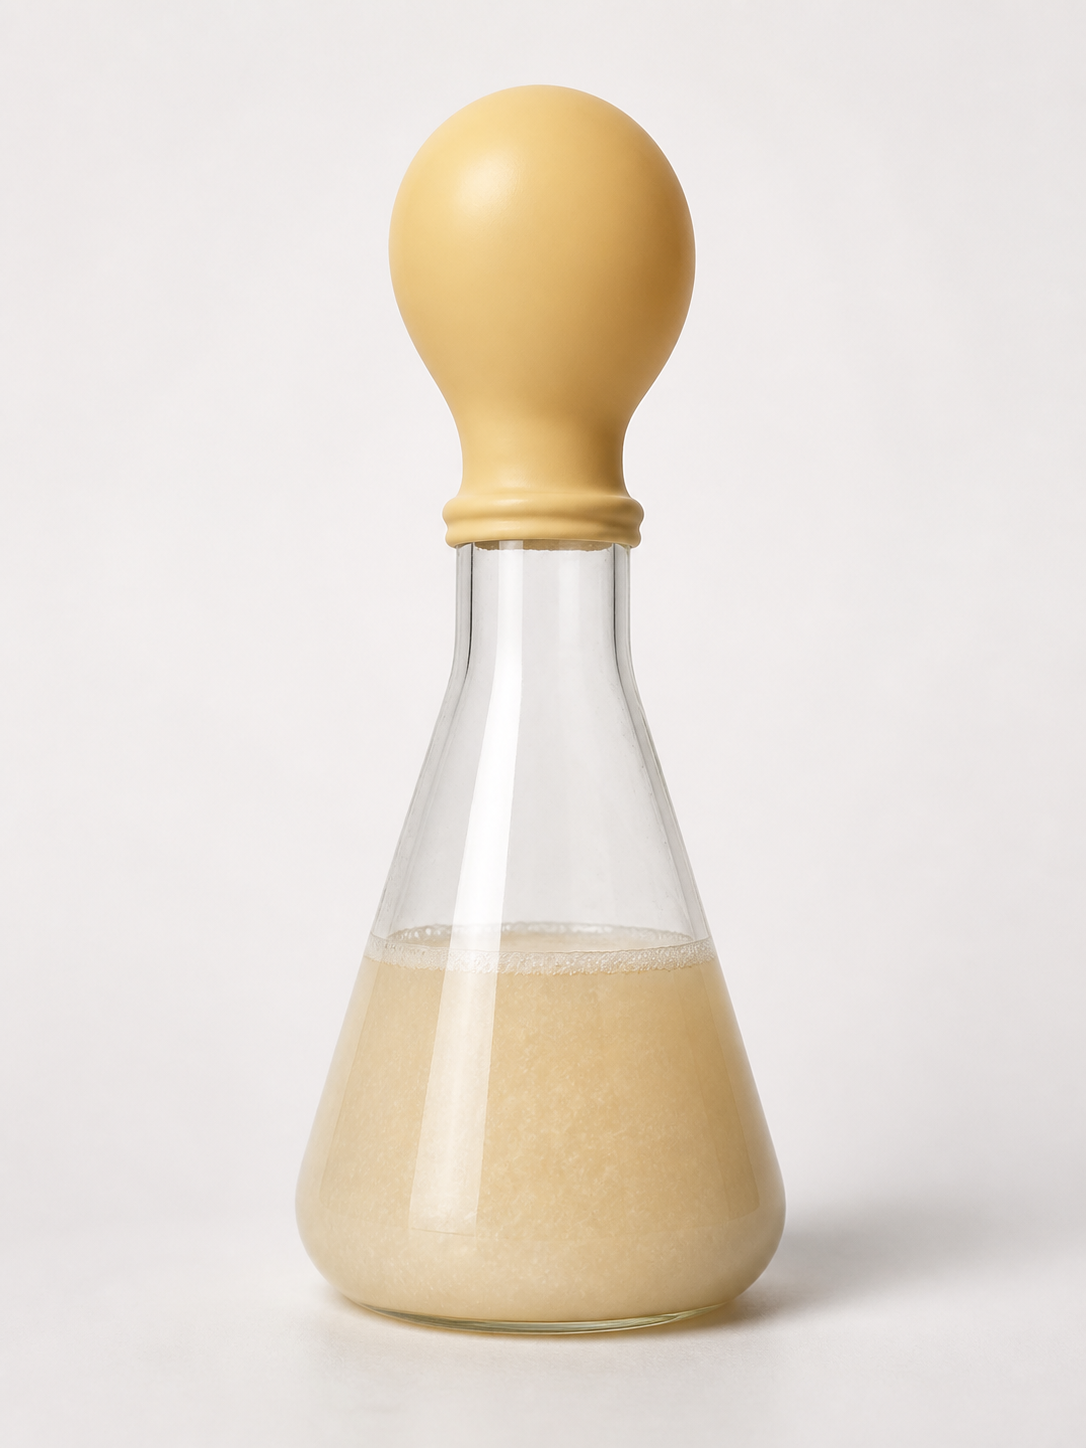
\includegraphics[width=0.36\linewidth]{images/book2/ai/g10-metab-yeast-balloon.png}

{\small Gist die suiker vergist in een kolf: de koolstofdioxide van de
alcoholische \omterm{def:g10:cell-metabolism:fermentation}{gisting} blaast de ballon op. Doordat er geen zuurstof in de
vloeistof zit, wordt de suiker slechts gedeeltelijk afgebroken en blijft
de ethanol achter.}
\end{omfigure}

\begin{example}[Gist met en zonder lucht]\label{ex:g10:cell-metabolism:pasteur}
Gist waar lucht doorheen wordt geblazen, gebruikt glucose spaarzaam en
groeit snel: zij ademt. Dezelfde gist in een afgesloten vat gebruikt
glucose gulzig, groeit weinig en maakt ethanol: zij vergist. Pasteur,
die dit in 1861 beschreef, noemde de \omterm{def:g10:cell-metabolism:fermentation}{gisting} "leven zonder lucht"; de
\omterm{def:g10:cells-common-unit:cell}{cellen} schakelen hun \omterm{def:g10:cell-metabolism:metabolism}{stofwisseling} om naar de route die hun omgeving
toelaat, en omdat de \omterm{def:g10:cell-metabolism:fermentation}{gisting} zo weinig energie per glucose oplevert,
moeten zij veel meer suiker doorwerken om te leven.
\end{example}

\begin{omfigure}
\begin{tikzpicture}[>=Stealth, font=\small,
  cell/.style={draw, rounded corners, thick, minimum height=1.5cm, text width=2.7cm, align=center},
  inp/.style={text width=2.3cm, align=right, anchor=east},
  outp/.style={text width=2.6cm, align=left, anchor=west}]
  \node[cell, fill=omMeth!12] (a) at (0,0) {\textbf{autotrofe cel}\\ bladgroenkorrels};
  \node[inp] (ai) at (-2.2,0) {$\mathrm{CO_2}$, $\mathrm{H_2O}$,\\ minerale zouten,\\ \emph{licht}};
  \node[outp] (ao) at (2.2,0) {organische stof\\ (glucose, zetmeel\dots)\\ $+ \mathrm{O_2}$};
  \draw[->] (ai) -- (a); \draw[->] (a) -- (ao);
  \node[cell, fill=omThm!10] (h) at (0,-3.2) {\textbf{elke cel}\\ mitochondriën};
  \node[inp] (hi) at (-2.2,-3.2) {organische stof\\ $+ \mathrm{O_2}$};
  \node[outp] (ho) at (2.2,-3.2) {$\mathrm{CO_2}$, $\mathrm{H_2O}$\\ $+$ energie (ATP, warmte)};
  \draw[->] (hi) -- (h); \draw[->] (h) -- (ho);
  \node[anchor=west, font=\small\itshape] at (8.6,0) {fotosynthese};
  \node[anchor=west, font=\small\itshape] at (8.6,-3.2) {ademhaling};
  \draw[->, gray, thick] (4.6,-0.7) to[bend left=35] node[right, font=\scriptsize, text width=3.6cm, align=left, xshift=2pt] {organische stof voedt de heterotrofen, en de ademhaling van de autotroof zelf} (4.6,-2.5);
\end{tikzpicture}

{\small De twee stromen van de celstofwisseling. De \omterm{def:g10:cell-metabolism:autotrophy}{fotosynthese} slaat
lichtenergie op in \omterm{def:g10:chemistry-of-life:mineral-organic}{organische stof}; de ademhaling, in elke \omterm{def:g10:cells-common-unit:cell}{cel}, maakt
haar weer vrij. Autotrofen doen beide; heterotrofen doen alleen het
tweede en moeten met \omterm{def:g10:chemistry-of-life:mineral-organic}{organische stof} worden gevoed.}
\end{omfigure}

\section{Wat de stofwisseling van een cel bepaalt}

\begin{proposition}[Genen en omgeving]\label{prop:g10:cell-metabolism:decides}
De \omterm{def:g10:cell-metabolism:metabolism}{stofwisseling} van een \omterm{def:g10:cells-common-unit:cell}{cel} hangt van twee dingen af: van haar
\emph{uitrusting} --- de \omterm{def:g10:cell-metabolism:metabolism}{enzymen} en \omterm{def:g10:cells-common-unit:organelle}{organellen} die haar \omterm{def:g10:universal-dna:gene}{genen} haar laten
bouwen, zodat een \omterm{def:g10:cells-common-unit:cell}{cel} zonder bladgroen nooit \omterm{def:g10:cell-metabolism:autotrophy}{fotosynthese} kan bedrijven
--- en van haar \emph{omgeving} --- licht, zuurstof, beschikbare
voedingsstoffen --- die bepaalt welke van de mogelijke routes werkelijk
loopt. Een gist ademt in de lucht en vergist zonder lucht; een
\emph{Euglena} is \omterm{def:g10:cell-metabolism:autotrophy}{autotroof} in het licht en \omterm{def:g10:cell-metabolism:autotrophy}{heterotroof} in het donker;
een wortelcel van een groene plant is haar hele leven \omterm{def:g10:cell-metabolism:autotrophy}{heterotroof},
gevoed door de bladeren.
\end{proposition}
\admitted

\begin{method}[Een stofwisselingsgrafiek lezen]\label{met:g10:cell-metabolism:trace}
Proeven met een zuurstofsensor geven een concentratie tegen de tijd.
\begin{enumerate}
  \item Stel vast wat er op elk gemarkeerd moment veranderde (lamp aan,
        substraat toegevoegd, zuurstof op).
  \item Lees de helling van elk recht stuk af: stijging gedeeld door
        looplengte, in \unit{mg/L} per minuut. Een positieve helling
        betekent netto zuurstofproductie, een negatieve netto verbruik.
  \item Bedenk dat een \omterm{def:g10:cells-common-unit:cell}{cel} die \omterm{def:g10:cell-metabolism:autotrophy}{fotosynthese} bedrijft ook ademt: de
        helling in het licht is productie min ademhaling, dus de
        werkelijke snelheid van de \omterm{def:g10:cell-metabolism:autotrophy}{fotosynthese} is de helling in het
        licht plus de grootte van de helling in het donker.
  \item Reken om als daarom wordt gevraagd: bij deze concentraties komt
        \qty{1}{mg/L} opgeloste zuurstof overeen met $1/32$ millimol
        per liter.
\end{enumerate}
\end{method}

\begin{example}[De werkelijke snelheid van de alg]\label{ex:g10:cell-metabolism:truerate}
In de figuur van \emph{Chlorella} stijgt de zuurstof met \qty{2.5}{mg/L}
in 5 minuten licht (helling $+0.5$) en daalt zij met \qty{0.5}{mg/L} in
5 minuten donker (helling $-0.1$). Ook in het licht verbruikt de
ademhaling \qty{0.1}{mg/L} per minuut, dus produceert de \omterm{def:g10:cell-metabolism:autotrophy}{fotosynthese}
$0.5 + 0.1 = \qty{0.6}{mg/L}$ per minuut: zes keer wat de ademhaling
gebruikt. De alg is netto producent van zuurstof en \omterm{def:g10:chemistry-of-life:mineral-organic}{organische stof}, en
daarom groeit zij.
\end{example}

\section{Oefeningen}

\begin{exercise}[$\star$]\label{exo:g10:cell-metabolism:1}
Definieer \omterm{def:g10:cell-metabolism:metabolism}{stofwisseling}, en zeg wat een \omterm{def:g10:cell-metabolism:metabolism}{enzym} is en wat het doet.
\end{exercise}

\begin{exercise}[$\star$]\label{exo:g10:cell-metabolism:2}
Schrijf de samenvattende vergelijking van de \omterm{prop:g10:cell-metabolism:respiration}{celademhaling} en die van de
\omterm{def:g10:cell-metabolism:autotrophy}{fotosynthese} op. In welk opzicht is de ene het omgekeerde van de andere,
en in welk opzicht niet?
\end{exercise}

\begin{exercise}[$\star$]\label{exo:g10:cell-metabolism:3}
Deel in als \omterm{def:g10:cell-metabolism:autotrophy}{autotroof} of \omterm{def:g10:cell-metabolism:autotrophy}{heterotroof}: een paddenstoel, een mos, een
wortelcel van een wortel, een chlorella, een yoghurtbacterie, een
menselijke spiercel.
\end{exercise}

\begin{exercise}[$\star$]\label{exo:g10:cell-metabolism:4}
Welk gas blaast in de proef met gist en ballon de ballon op, welk
vloeibaar product hoopt zich op, en wat ontbreekt er in de kolf dat de
afloop zou veranderen?
\end{exercise}

\begin{exercise}[$\star$]\label{exo:g10:cell-metabolism:5}
Waarom laat gekookte lever waterstofperoxide niet meer schuimen?
\end{exercise}

\begin{exercise}[$\star\star$]\label{exo:g10:cell-metabolism:6}
In de figuur met gist daalt de zuurstof tussen minuut 3 en minuut 10 van
\qty{7.9}{mg/L} naar \qty{0.9}{mg/L}. Bereken de snelheid van de
ademhaling in \unit{mg/L} per minuut. Waarom vlakt de kromme na minuut
10 af, en wat doet de gist dan?
\end{exercise}

\begin{exercise}[$\star\star$]\label{exo:g10:cell-metabolism:7}
Chlorella vertoont in het licht een zuurstofhelling van $+0.8$
\unit{mg/L} per minuut, en in het donker $-0.2$. Bereken de snelheid van
de \omterm{def:g10:cell-metabolism:autotrophy}{fotosynthese}.
\end{exercise}

\begin{exercise}[$\star\star$]\label{exo:g10:cell-metabolism:8}
Een \omterm{def:g10:cells-common-unit:cell}{cel} ademt \qty{18}{g} glucose. Hoeveel zuurstof gebruikt zij daarbij
en hoeveel koolstofdioxide geeft zij af? (Molaire massa's: glucose
\qty{180}{g/mol}, $\mathrm{O_2}$ \qty{32}{g/mol}, $\mathrm{CO_2}$
\qty{44}{g/mol}.)
\end{exercise}

\begin{exercise}[$\star\star$]\label{exo:g10:cell-metabolism:9}
Kiemende erwten in een thermosfles verhogen de temperatuur ervan in een
dag met \qty{4}{\celsius}; gekookte erwten niet. Verklaar beide
uitkomsten, en zeg waarom de fles niet luchtdicht mag worden afgesloten.
\end{exercise}

\begin{exercise}[$\star\star$]\label{exo:g10:cell-metabolism:10}
Een groen blad wordt 48 uur in het donker gehouden, daarna wordt de
helft ervan met zwart papier afgedekt en gaat de plant een dag in de
zon. Er wordt jood opgebracht. Voorspel en verklaar het resultaat op
elke helft, en zeg waarom de 48 uur donker nodig waren.
\end{exercise}

\begin{exercise}[$\star\star$]\label{exo:g10:cell-metabolism:11}
Leg uit waarom gist in een afgesloten vat per \omterm{def:g10:cells-common-unit:cell}{cel} veel sneller suiker
verbruikt dan gist waar lucht doorheen wordt geblazen.
\end{exercise}

\begin{exercise}[$\star\star\star$]\label{exo:g10:cell-metabolism:12}
De spieren van een sprinter worden na een race van 400 meter pijnlijk en
zuur. Leg uit wat er in de spiercellen gebeurde, waarom het gebeurde, en
waarom de spieren van diezelfde loper bij een rustige duurloop niet zuur
worden.
\end{exercise}

\begin{exercise}[$\star\star\star$]\label{exo:g10:cell-metabolism:13}
Een \emph{Euglena} die een maand in het donker met organisch voedsel
wordt gehouden, verliest haar \omterm{def:g10:cells-common-unit:organelle}{bladgroenkorrels}, maar haar nakomelingen
krijgen ze in het licht terug. Welke van de twee factoren uit
\cref{prop:g10:cell-metabolism:decides} is veranderd en welke niet? Wat
bewijst het herstel over de \omterm{def:g10:universal-dna:gene}{genen} van de \omterm{def:g10:cells-common-unit:cell}{cel}?
\end{exercise}

\begin{exercise}[$\star\star\star$]\label{exo:g10:cell-metabolism:14}
Een afgesloten aquarium bevat water, een slak en een waterplant, in het
licht. Leg uit hoe beide organismen maandenlang kunnen overleven, wat
elk aan de ander levert, en wat er gebeurt als het aquarium in het
donker wordt gezet.
\end{exercise}

\begin{exercise}[$\star\star\star$]\label{exo:g10:cell-metabolism:15}
De ademhaling van één glucose levert ongeveer 30 ATP op, de \omterm{def:g10:cell-metabolism:fermentation}{gisting} 2.
Een gistcel heeft per minuut een vast aantal ATP nodig om te leven.
Bereken hoeveel keer meer glucose zij per minuut moet verbruiken als zij
vergist; leg vervolgens uit waarom brouwers lucht uit hun vaten houden,
ook al "verspilt" dat suiker.
\end{exercise}

\section{Probleem: Het vat van de wijnmaker}

\begin{problem}[{Weekendprobleem --- een vat druivensap overgelaten aan
de gist: de alcohol die het zal bevatten, het gas dat het zal afgeven, de
warmte die het zal maken, en waarom een kelder gevaarlijk kan zijn}]
\label{pb:g10:cell-metabolism:1}
Druivensap (most) bevat ongeveer \qty{200}{g} suiker per liter, die wij
als glucose opvatten, en geen opgeloste zuurstof zodra het vat is
gesloten. Molaire massa's: glucose \qty{180}{g/mol}, ethanol
$\mathrm{C_2H_5OH}$ \qty{46}{g/mol}, koolstofdioxide \qty{44}{g/mol},
zuurstof \qty{32}{g/mol}. De dichtheid van ethanol is \qty{0.79}{g/mL}.
Eén mol gas neemt bij keldertemperatuur ongeveer \qty{24}{L} in. Het vat
bevat \qty{1000}{L}.

\medskip
\noindent\textbf{Deel I --- Wat de gist maakt.}
\begin{enumerate}
  \item Welke route volgt de gist in het gesloten vat, en waarom?
        Schrijf haar vergelijking op.
  \item Hoeveel mol glucose bevat één liter most?
  \item Bereken de massa ethanol die per liter wordt gemaakt, dan het
        volume ervan, en dan het alcoholgehalte van de wijn in
        volumeprocent.
  \item Bereken de massa koolstofdioxide die per liter most wordt
        gemaakt, en het volume ervan als gas.
  \item Welk volume koolstofdioxide komt er voor het hele vat vrij?
        Vergelijk met het volume van een kelder van \qty{4}{m} bij
        \qty{6}{m} bij \qty{2.5}{m}.
\end{enumerate}

\medskip
\noindent\textbf{Deel II --- Als de gist lucht had.}
\begin{enumerate}[resume]
  \item Schrijf de vergelijking op die de gist zou volgen als de most
        voortdurend werd belucht.
  \item Bereken de massa zuurstof die nodig is om de suiker van één
        liter most te verademen, en de massa koolstofdioxide die
        vrijkomt.
  \item Vergelijk de koolstofdioxide van vraag 7 met die van vraag 4, en
        verklaar het verschil vanuit de mate waarin de glucose wordt
        afgebroken.
  \item De ademhaling levert ongeveer 30 ATP per glucose op en de
        \omterm{def:g10:cell-metabolism:fermentation}{gisting} 2. Als de gist in beide gevallen evenveel ATP nodig
        heeft, in welk geval gaat de suiker dan langer mee, en met welke
        factor?
  \item Leg uit waarom een wijnmaker toch lucht buiten houdt.
\end{enumerate}

\medskip
\noindent\textbf{Deel III --- De warmte van het vat.}
De \omterm{def:g10:cell-metabolism:fermentation}{gisting} geeft ongeveer \qty{70}{kJ} warmte per mol glucose af;
\qty{1}{kg} water \qty{1}{\celsius} verwarmen kost \qty{4.2}{kJ}.
\begin{enumerate}[resume]
  \item Bereken de warmte die per liter most vrijkomt, en vervolgens die
        voor het hele vat.
  \item Als er niets van ontsnapte, met hoeveel zou de temperatuur van
        het vat dan stijgen? (Neem de most als water.)
  \item \omterm{def:g10:cell-metabolism:metabolism}{Enzymen} van gist worden boven ongeveer \qty{40}{\celsius}
        vernield. Zou een ongekoeld vat, beginnend bij
        \qty{20}{\celsius}, het overleven? Wat zegt dat over waarom
        grote vaten worden gekoeld?
  \item Leg met \cref{prop:g10:cell-metabolism:enzymes} uit waarom
        warmte de \omterm{def:g10:cell-metabolism:fermentation}{gisting} stillegt, ook al is de suiker er nog.
  \item De ademhaling zou ongeveer \qty{2870}{kJ} per mol hebben
        vrijgemaakt. Waar blijft de energie die de \omterm{def:g10:cell-metabolism:fermentation}{gisting} \emph{niet}
        vrijmaakt?
\end{enumerate}

\medskip
\noindent\textbf{Deel IV --- De kelder.}
\begin{enumerate}[resume]
  \item Koolstofdioxide is dichter dan lucht. Waar in de kelder hoopt zij
        zich op, en waarom is een laag gedragen brandende kaars een
        klassieke veiligheidsproef?
  \item Op welke route zouden de \omterm{def:g10:cells-common-unit:cell}{cellen} van een werknemer zonder
        zuurstof overschakelen --- en waarom kan een menselijk lichaam
        daar niet langer dan enkele minuten van leven?
  \item De \omterm{def:g10:cell-metabolism:fermentation}{gisting} stopt vanzelf zodra de alcohol ongeveer 15\%
        volumeprocent bereikt. Stel een verklaring voor in termen van de
        \omterm{def:g10:cell-metabolism:metabolism}{enzymen} van de gist.
  \item Brooddeeg gebruikt dezelfde gist gedurende een uur. Wat zit er
        in de bellen van de kruim, en waar is de ethanol na het bakken
        gebleven?
  \item Geef het resultaat: voor één liter most het alcoholgehalte en het
        volume gas dat wordt gemaakt --- en het ene feit uit de
        \omterm{def:g10:cell-metabolism:metabolism}{stofwisseling} dat beide verklaart.
\end{enumerate}
\end{problem}
